% Cruise Speed Chart - Wheel Pants ON
\begin{figure}[t]
% \addcontentsline{toc}{section}{Figure \ref{Cruise-speed} Cruise Speed}
\addcontentsline{toc}{section}{CRUISE SPEED}
\begin{center}
\begin{perfhdr}CRUISE SPEED\\
\end{perfhdr}

\begin{minipage}{5in}
  \begin{flushleft}
    CONDITIONS:\\
    Wheel Pants and Gear Leg Fairings ON\\
    Standard atmosphere.\\
    Mixture set to best power for 75\% power.\\
    Mixture set to 50\textdegree F lean of peak EGT for 65\% and 55\% power, except mixture set to best power if more than 2600 rpm required with mixture set lean of peak EGT.\\
    Full throttle, but no less than 2100 rpm.\\
    Speed vs RPM lines are at full throttle, with mixture set to best power or 50 deg F Lean of Peak EGT.
    \end{flushleft}
\end{minipage}\\
\vspace{5ex}

% GNUPLOT: LaTeX picture with Postscript
\begingroup
  \makeatletter
  \providecommand\color[2][]{%
    \GenericError{(gnuplot) \space\space\space\@spaces}{%
      Package color not loaded in conjunction with
      terminal option `colourtext'%
    }{See the gnuplot documentation for explanation.%
    }{Either use 'blacktext' in gnuplot or load the package
      color.sty in LaTeX.}%
    \renewcommand\color[2][]{}%
  }%
  \providecommand\includegraphics[2][]{%
    \GenericError{(gnuplot) \space\space\space\@spaces}{%
      Package graphicx or graphics not loaded%
    }{See the gnuplot documentation for explanation.%
    }{The gnuplot epslatex terminal needs graphicx.sty or graphics.sty.}%
    \renewcommand\includegraphics[2][]{}%
  }%
  \providecommand\rotatebox[2]{#2}%
  \@ifundefined{ifGPcolor}{%
    \newif\ifGPcolor
    \GPcolorfalse
  }{}%
  \@ifundefined{ifGPblacktext}{%
    \newif\ifGPblacktext
    \GPblacktexttrue
  }{}%
  % define a \g@addto@macro without @ in the name:
  \let\gplgaddtomacro\g@addto@macro
  % define empty templates for all commands taking text:
  \gdef\gplbacktext{}%
  \gdef\gplfronttext{}%
  \makeatother
  \ifGPblacktext
    % no textcolor at all
    \def\colorrgb#1{}%
    \def\colorgray#1{}%
  \else
    % gray or color?
    \ifGPcolor
      \def\colorrgb#1{\color[rgb]{#1}}%
      \def\colorgray#1{\color[gray]{#1}}%
      \expandafter\def\csname LTw\endcsname{\color{white}}%
      \expandafter\def\csname LTb\endcsname{\color{black}}%
      \expandafter\def\csname LTa\endcsname{\color{black}}%
      \expandafter\def\csname LT0\endcsname{\color[rgb]{1,0,0}}%
      \expandafter\def\csname LT1\endcsname{\color[rgb]{0,1,0}}%
      \expandafter\def\csname LT2\endcsname{\color[rgb]{0,0,1}}%
      \expandafter\def\csname LT3\endcsname{\color[rgb]{1,0,1}}%
      \expandafter\def\csname LT4\endcsname{\color[rgb]{0,1,1}}%
      \expandafter\def\csname LT5\endcsname{\color[rgb]{1,1,0}}%
      \expandafter\def\csname LT6\endcsname{\color[rgb]{0,0,0}}%
      \expandafter\def\csname LT7\endcsname{\color[rgb]{1,0.3,0}}%
      \expandafter\def\csname LT8\endcsname{\color[rgb]{0.5,0.5,0.5}}%
    \else
      % gray
      \def\colorrgb#1{\color{black}}%
      \def\colorgray#1{\color[gray]{#1}}%
      \expandafter\def\csname LTw\endcsname{\color{white}}%
      \expandafter\def\csname LTb\endcsname{\color{black}}%
      \expandafter\def\csname LTa\endcsname{\color{black}}%
      \expandafter\def\csname LT0\endcsname{\color{black}}%
      \expandafter\def\csname LT1\endcsname{\color{black}}%
      \expandafter\def\csname LT2\endcsname{\color{black}}%
      \expandafter\def\csname LT3\endcsname{\color{black}}%
      \expandafter\def\csname LT4\endcsname{\color{black}}%
      \expandafter\def\csname LT5\endcsname{\color{black}}%
      \expandafter\def\csname LT6\endcsname{\color{black}}%
      \expandafter\def\csname LT7\endcsname{\color{black}}%
      \expandafter\def\csname LT8\endcsname{\color{black}}%
    \fi
  \fi
  \setlength{\unitlength}{0.0500bp}%
  \begin{picture}(7200.00,5040.00)%
    \gplgaddtomacro\gplbacktext{%
      \csname LTb\endcsname%
      \put(1342,704){\makebox(0,0)[r]{\strut{}0}}%
      \csname LTb\endcsname%
      \put(1342,1286){\makebox(0,0)[r]{\strut{}2,000}}%
      \csname LTb\endcsname%
      \put(1342,1867){\makebox(0,0)[r]{\strut{}4,000}}%
      \csname LTb\endcsname%
      \put(1342,2449){\makebox(0,0)[r]{\strut{}6,000}}%
      \csname LTb\endcsname%
      \put(1342,3030){\makebox(0,0)[r]{\strut{}8,000}}%
      \csname LTb\endcsname%
      \put(1342,3612){\makebox(0,0)[r]{\strut{}10,000}}%
      \csname LTb\endcsname%
      \put(1342,4193){\makebox(0,0)[r]{\strut{}12,000}}%
      \csname LTb\endcsname%
      \put(1342,4775){\makebox(0,0)[r]{\strut{}14,000}}%
      \csname LTb\endcsname%
      \put(1474,484){\makebox(0,0){\strut{} 140}}%
      \csname LTb\endcsname%
      \put(2148,484){\makebox(0,0){\strut{} 145}}%
      \csname LTb\endcsname%
      \put(2823,484){\makebox(0,0){\strut{} 150}}%
      \csname LTb\endcsname%
      \put(3497,484){\makebox(0,0){\strut{} 155}}%
      \csname LTb\endcsname%
      \put(4172,484){\makebox(0,0){\strut{} 160}}%
      \csname LTb\endcsname%
      \put(4846,484){\makebox(0,0){\strut{} 165}}%
      \csname LTb\endcsname%
      \put(5520,484){\makebox(0,0){\strut{} 170}}%
      \csname LTb\endcsname%
      \put(6195,484){\makebox(0,0){\strut{} 175}}%
      \csname LTb\endcsname%
      \put(6869,484){\makebox(0,0){\strut{} 180}}%
      \put(308,2739){\rotatebox{-270}{\makebox(0,0){\strut{}Altitude (ft)}}}%
      \put(4171,154){\makebox(0,0){\strut{}Cruise Speed (KTAS)}}%
      \put(5318,1373){\rotatebox{50}{\makebox(0,0)[l]{\strut{}75\% Power}}}%
      \put(4509,1727){\rotatebox{50}{\makebox(0,0)[l]{\strut{}65\% Power}}}%
      \put(3093,2158){\rotatebox{50}{\makebox(0,0)[l]{\strut{}55\% Power}}}%
      \put(4172,3874){\makebox(0,0){\strut{}\Large\textcolor{red}{FROM ANALYSIS OF CAFE DATA}\normalsize}}%
      \put(4172,3292){\makebox(0,0){\strut{}\Large\textcolor{red}{PENDING FLIGHT TEST}\normalsize}}%
    }%
    \gplgaddtomacro\gplfronttext{%
    }%
    \gplbacktext
    \put(0,0){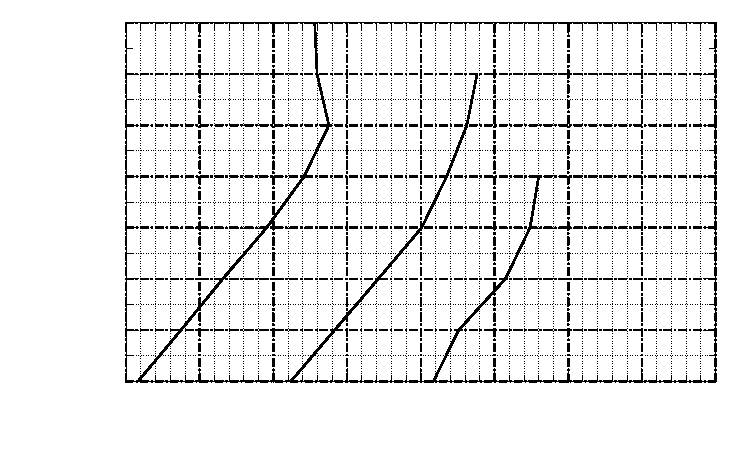
\includegraphics{../graphs/cruise_speed}}%
    \gplfronttext
  \end{picture}%
\endgroup
\end{center}  % for gnuplot epslatex, latex or pslatex mode
\caption{Cruise Speed}
\label{Cruise-speed}
\end{figure}


